\documentclass[12pt,english]{article}
\usepackage{mathptmx}

\usepackage{color}
\usepackage[dvipsnames]{xcolor}
\definecolor{darkblue}{RGB}{0.,0.,139.}

\usepackage[top=1in, bottom=1in, left=1in, right=1in]{geometry}

\usepackage{amsmath}
\usepackage{amstext}
\usepackage{amssymb}
\usepackage{setspace}
\usepackage{lipsum}

\usepackage[authordate]{natbib}
\bibliographystyle{chicago}
\usepackage{url}
\usepackage{booktabs}
\usepackage[flushleft]{threeparttable}
\usepackage{graphicx}
\usepackage[english]{babel}
\usepackage{pdflscape}
\usepackage[unicode=true,pdfusetitle,
 bookmarks=true,bookmarksnumbered=false,bookmarksopen=false,
 breaklinks=true,pdfborder={0 0 0},backref=false,
 colorlinks,citecolor=black,filecolor=black,
 linkcolor=black,urlcolor=black]
 {hyperref}
\usepackage[all]{hypcap} % Links point to top of image, builds on hyperref
\usepackage{breakurl}    % Allows urls to wrap, including hyperref

\linespread{2}

\begin{document}

\begin{singlespace}
\title{Quantity over Quality? Analyzing Journal-Level Citations with scite}
\end{singlespace}

\author{Mason Ross Hayes\thanks{Department of Economics, University of Oklahoma.\
E-mail~address:~\href{mailto:masonrhayes@ou.edu}{masonrhayes@ou.edu}}}

\date{\today}

\maketitle

\begin{abstract}
\begin{singlespace}
Gathering journal-level citation data from the scite API through the sciteR package, which I created for this paper, I find that journal quality varies widely across disciplines. Mathematics, physics, and chemistry have a much higher scite journal index than do medicine and economics, for example.
Using a sample of 589 journals across the disciplines of math, physics, chemistry, biology, business, economics, and medicine, I attempt to use a machine-learning model to classify each journal by subject according to its scite journal index (sji).
\end{singlespace}

\end{abstract}
\vfill{}


\pagebreak{}


\section{Introduction}\label{sec:intro}
Mainstream citation indices such as impact factor or h-index do not incorporate the author's intent in making the citations. For example, if Article 1 cites Article 2 in order question the findings, methods, or data sources of Article 2, this nonetheless counts as a citation for Article 2. In other words, any citation is a good citation. \href{https://scite.ai}{scite} provides a way to correct for this inaccurate measurement by using their deep-learning model to categorize a citation as supporting, contradicting, or simply mentioning. This provides a much more comprehensive look at not only the quantity but also the quality of citations. This quality is measured using the scite journal index, or sji, which is calculated as the number of supporting citations divided by the total number of supporting plus contradicting citations:

\begin{equation}
    sji = \frac{\text{supporting citations}}{\text{supporting + contradicting citations}}
\end{equation}

This article is divided into 4 main sections in addition to this introduction. What follows is a literature review of the relevant research that has already been done on citation indexing, which is quite extensive. Using citation counts as a measure of prestige or productivity has long been questioned, but nonetheless remains the primary method of ranking journals, authors, and universities. A new, modern method of ranking is necessary, and scite provides a great step towards a future where rankings are controlled for scientific value and accuracy.

\section{Literature Review}\label{sec:litreview}

Citation counts are an important part of academic work; for many researchers across every field, a higher citation count can mean more funding, more prestige, and more respect in their field. Various papers have studied the effects of citations and they way that citation methods vary across fields. 

While higher citation counts are generally interpreted as higher quality work, the various other factors that influence an author's decision to cite another author make the pure count of citations inaccurate. Other than simply making errors which some future authors later contradict (which, considering only citation count, would be a benefit for a researcher), some researchers and even entire journals have been found to engage in citation manipulation, or purposely and artificially increasing the citation count for a given article, journal, or author \citep{bartneck_detecting_2011, perbal_disastrous_2017,  fire_over-optimization_2019}.

Manipulating one's own h-index has been shown to be quite easy \citep{duyx_scientific_2017}. Given the payoff -- pay raises, promotions, more research funding, faster track to tenure, and more prestige in one's field -- the manipulation of citation counts is expected \citep{patience_citation_2017}. A detailed overview of the different types of unethical citation strategies that some authors, journals, or disciplines often use has been done by \cite{moustafa_aberration_2016}.

There is also a strong positive-result bias in all scientific or academic publishing; negative results or results that do not align with the available literature often go unpublished and forgotten. This positive-result bias has been shown to be most prevalent in biological and medical science, and least prevalent in the natural sciences such as physics or chemistry \citep{duyx_scientific_2017}. Additionally, \cite{duyx_scientific_2017} found that "articles in which the authors explicitly conclude to have found support for their hypothesis were cited 2.7 times as often."

scite's classifications of citations as supporting or contradicting can help researchers understand if a particular paper's traditional citation indices have been manipulated or are biased, since this type of index is much less susceptible to manipulation or bias. It can also provide greater value to publishing non-significant results, since non-significant results could later be contradicted or supported accordingly, and help to remove the strong positive result so prevalent in scientific research. 

Finally, this new approach to citation reporting is important for the real-world implications it can have, particularly in the field of biomedical science. Findings that propose some new medical treatment can be subsequently contradicted based on new, higher-quality research; smart citations allow this type of updating.


\section{Data}\label{sec:data}

The primary data for this research is scite's journal-level citation data, which includes the scite journal index, total citations, supporting citations, and contradicting citations \footnote{To fully understand how each citation is classified as supporting or contradicting, please see \href{https://scite.ai/#learn-more}{scite's explanation}}. ISSNs were collected through Ulrich's database, Wikipedia's list of top scientific journals by category, and EconLit for economics journals. Collecting the issn of each journal manually can prove very tedious -- ISSNs were collected primarily from ulrich's database and from EconLit, then filtered by active journals in the disciplines of physics, chemistry, biology, medicine, or economics. To make this code and findings of this paper reproducible, an Excel sheet of the journals along with all of their citation data is openly available (see the project repository).

Each journal was collected along with its respective ISSN, which is necessary to get the data from scite. The scite API is quite new, so no standardized way of interacting with it existed until this paper. To facilitate future research, I have created an R package, \href{https://github.com/masonrhayes/sciteR}{sciteR}, to interface with the API. All necessary documentation can be found at the github page for the package, as well as in the appendix. This new package will allow for much easier and quicker reproduction of the findings from this article; currently, according to scite, some of the caveats of their API are:
\begin{itemize}
    \item If an ISSN is not in the system, it won’t be included in the response
    \item When a journal does not meet the 500 supporting + contradicting threshold, the value will simply be NULL
    \item The scite API is currently unauthenticated, but this may change.
\end{itemize}


For each journal, the "subject" category was added manually according to the journal's title or, if more information was necessary, from the journal's description. Journals that publish in various disciplines or which have no clearly defined single subject were put into a category of "other" and subsequently dropped from the sample. Most of the "other" journals were social science journals. While future research on these social science journals would be valuable, it is not the focus of this paper; rather, I seek to compare primarily economics or business journals to the main disciplines of the natural and life sciences. In a later section of this paper, I consider the effects of broadening the categories into science, social science, medicine, or math. This is done in order to overcome many of the arbitrary classifications; biology and chemistry journals, for example, often have significant overlap in their research focus, as do physics journals and chemistry journals.

The data used for the analysis in this paper is a data frame of citation data from scite, accessed through the scite API using the sciteR package. Table \ref{tab:descriptives} contains summary statistics.


\section{Empirical Methods}\label{sec:methods}

I consider two models for the sake of comparison: a standard linear regression model, and a machine-learning classification model using mlr3.

In particular, the first linear model I propose is intended to quantify the systematic differences between journals of different disciplines. I hypothesize that natural science or "hard science" journals such as mathematics, physics, or chemistry will have higher SJIs than life sciences or medicine, and that the social science journals will have the lowest SJIs among these disciplines.

I make this hypothesis for two reasons: research in the social sciences like economics, business, psychology, or political science are much harder to replicate than are findings in the sciences. Secondly, they are more prone to bias through differing ideologies within their respective fields \citep{duyx_scientific_2017}.

The proposed linear model is:
\begin{equation}
    sji = \beta_0 + \beta_1 t + \beta_2 b + \beta_3 c + \beta_4 e + \beta_5 m_1 + \beta_6 m_2 + \beta_7 p + \epsilon
\end{equation}
where $t =$ total citations, with binary variables $b =$ business, $c =$ chemistry, $e =$ economics, $m_1 =$ math, $m_2 =$ medicine, and $p =$ physics.

Secondly, the machine learning model attempts to classify a journal into one of the 7 subject categories given the sji across all years, and each citation variable (total, supporting, mentioning, contradicting). I use the mlr3 package in R to train the model on 80\% of the sample, and test the model on the remaining 20\% of the sample. The code to reproduce these findings can be found at the respective github repository for this paper, as well as in the appendix.

\section{Research Findings}\label{sec:results}
The results from the linear model are reported in Table \ref{tab:estimates}. With this model alone, the initial hypothesis is mostly correct; however, medicine journals do far worse than expected. Compared to all other journals in this sample (N = 589), medicine journals have the lowest sji ($\beta = -0.042$ lower than the sji for biology journals). The sji is highest for math journals, which have a minumum sji of 0.89 and an average of 0.95, a full 10 points higher than medicine journals. As anticipated, physics and chemistry journals also have higher sjis than social or life science journals. 

The journal with the highest sji in the sample is the \textit{Mathematical Proceedings of the Cambridge Philosophical Society} with an sji of 0.979, and the journal with the lowest sji is the \textit{Journal of Veterinary Internal Medicine} with an sji of 0.779. Of the bottom 10\% of journals according to sji, 38 out of 58 of them (65\%) are medical journals, and 15 out of 58 (26\%) are biology journals. Of the top 10\% of journals according to sji, 26 out of 58 of them are math journals. This means that more than 80\% of the math journals in this dataset are in the top 10\% by sji. 

In line with the literature that has called into question the value of measuring simple citation counts, there is \textit{no significant correlation} between sji and total citation count (see Figure \ref{fig:fig3}. The top cited 10\% of journals have an average sji of 0.892, which is only slightly higher than the average sji across the entire sample, 0.886.

A visualization of the differences in sji across the disciplines can be seen in Figure \ref{fig:fig1}

The machine learning model was not able to classify each journal by subject with an appropriate level of accuracy (see Table \ref{tab:confusion}). Physics journals, for example, were often confused with biology journals. The model was able to predict well if a journal was an economics journal: it correctly identified 13 out of 16 economics journals (81\%). It also correctly identified 5 out of 8 math journals, or about 63\%. The remaining results are far from impressive; less than half of biology, chemistry, medicine, or business journals were correctly identified. Physics journals in particular were almost always classified as biology or chemistry journals. Business journals, by sji only, do not seem to be any different than economics journals; they are very unlikely to have an sji higher than 0.90, and the majority of their density lies between 0.83 and 0.90. The fact that most business journals were classified as economics journals then is unsurprising, particularly due to the general overlap of the two fields. 

These results make sense after taking a look at Figure \ref{fig:fig2}. If a journal has an SJI below 0.825, for example, it is almost certainly a biology or medicine journal. With an SJI between 0.90 and 0.95, however, it becomes much more difficult to determine the subject due to the large overlap -- it is almost equally likely to be a physics, chemistry, or biology journal.


\section{Empirical Methods 2: Considering More General Categories}

It could be argued that some of the classification are arbitrary; is a biological chemistry journal biology, or is it chemistry? Is the \textit{Journals of Gerontology Series A: Biological Sciences \& Medical Sciences} a medicine journal, or is it biology? These overlaps in fields make such specific classifications much less meaningful. I think it is more important to consider, then, how accurately the model predicts either the true subject or the next-best-subject. For example, if all medicine journals are classified as medicine or biology, this could still be a successful and useful result.

In an attempt to make the results more generalizable and to avoid the possibility of 'overclassification' in which multidisciplinary journals are arbitrarily classified into one or another category, I have combined physics, chemistry, and biology journals into one group, science. Economics, businesses and other social science journals were all classified simply as social science. The categories of medicine and math remain unchanged.

The same model frameworks were used to analyze this newly classified data; a linear model to estimate the parameters determining sji, and a machine learning model to classify each journal by subject.

\section{Results 2: Reclassified Subjects}

The changes in sji distributions following this re-categorization can be seen in Figure \ref{fig:fig4}. Combining related subjects into one category prevents the high levels of overlap that occurs when subjects are over-classified. 

Table \ref{tab:confusion_reclassified} shows the confusion matrix of the machine learning model using the new, more general categories. Its prediction accuracy is much higher: it correctly identifies 47 out of 56 science journals, or 84\%. 27 out of 33 social science journals (82\%) were correctly identified. The majority of medicine journals were not accurately identified; as many were classified as social science as were classified as medicine. Also, more were identified as science than as medicine.

For the same reasons as before, the confusion between medicine journals and science journals is expected due to the many shared characteristics of the journals. Medicine is kept as a separate category here only for illustrative purposes and because medicine journals have a particularly low sji on average.

\section{Conclusion}\label{sec:conclusion}

In this paper I have demonstrated that the citation quality of academic journals, as measured by the scite journal index, varies across disciplines. Journals in the "hard sciences" such as math, physics, or chemistry have much higher sji than social science journals such as economics or business. As illustrated in the paper, medical journals fare far worse than what I supposed would be comparable journals in the fields of biology or chemistry. Medicine journals have an average SJI 0.10 points lower than math journals, and about 0.05 points lower than science journals.

The models I have used do not provide insight into why this might be the case; research from \cite{duyx_scientific_2017} and others indicates that some fields are more susceptible to citation bias or unethical citation practices. There is also the possibility that medical journals receive more citations and are held to different standards of evidence due to some unique characteristics of the discipline \citep{patience_citation_2017}. There is no evidence that total citations is a good explanation of SJI for any of the journals in this data set (see Figure \ref{fig:fig3}). For medicine journals, the correlation between total citations and SJI is only 0.096. 

The study of citation indices is not new; known as scientometrics, bibliometrics, or journalology, researchers have long understood the downsides of standard citation metrics and have sought a new method of evaluating the quality of articles in a way that can be generalized across disciplines \citep{garfield_evolution_2007}. Hopefully, the continued expansion of scite's innovating journal metrics can be used for future research to create a more clear and transparent way to rank and categorize academic journals.

\vfill
\pagebreak{}
\begin{spacing}{1.0}
\bibliography{DSFinalProject.bib}
\addcontentsline{toc}{section}{References}
\end{spacing}

\vfill
\pagebreak{}
\clearpage

%========================================
% FIGURES AND TABLES 
%========================================
\section*{Figures and Tables}\label{sec:figTables}
\addcontentsline{toc}{section}{Figures and Tables}
%----------------------------------------
% Figure 1
%----------------------------------------
\begin{figure}[ht]
\centering
\bigskip{}
\includegraphics[width=.95\linewidth]{sji_density_initial-transparent.png}
\caption{sji Density by Subject. N = 589. See Figure \ref{fig:fig2} for a clearer visualization.}
\label{fig:fig1}
\end{figure}

%----------------------------------------
% Figure 2
%----------------------------------------
\begin{figure}[ht]
\centering
\bigskip{}
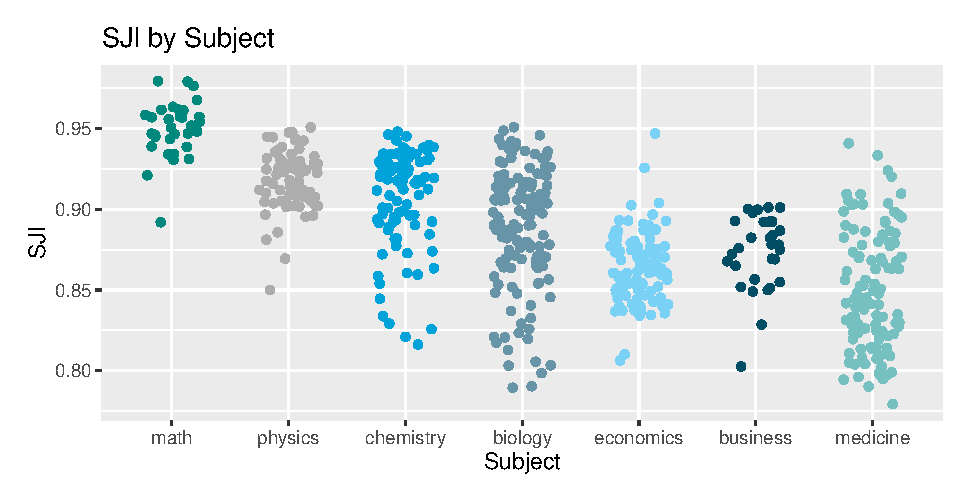
\includegraphics[width=.9\linewidth]{sji_by_subject_jitter.eps}
\caption{sji Distribution by Subject . N = 589}
\label{fig:fig2}
\end{figure}

%----------------------------------------
% Figure 3
%----------------------------------------

\begin{figure}
    \centering
    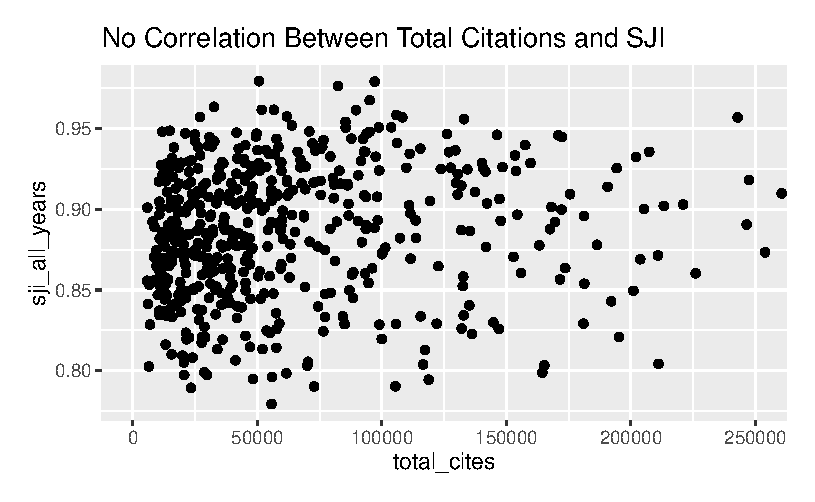
\includegraphics{total_cites_vs_sji.eps}
    \caption{Correlation = 0.032}
    \label{fig:fig3}
\end{figure}

%----------------------------------------
% Figure 4
%----------------------------------------

\begin{figure}
    \centering
    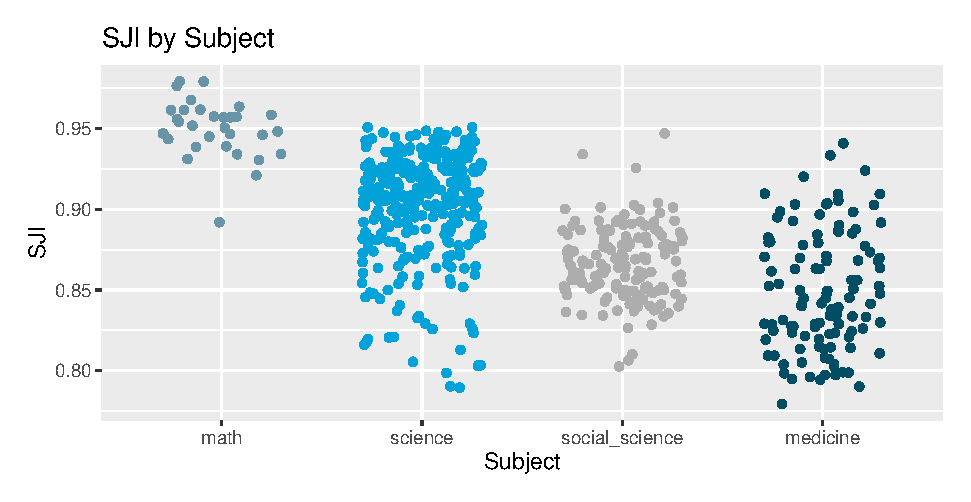
\includegraphics{sji_by_subject_reclassified.eps}
    \caption{Combining Related Subjects into One Category}
    \label{fig:fig4}
\end{figure}

%----------------------------------------
% Figure 5
%----------------------------------------

\begin{figure}
    \centering
    \includegraphics{sji_density_reclassified-transparent.png}
    \caption{Categories Are More Clearly Separated when Generalized}
    \label{fig:fig5}
\end{figure}

%----------------------------------------
% Table 1
%----------------------------------------
\begin{table}[!htbp] \centering 
  \caption{Summary Statistics of Scite Data} 
  \label{tab:descriptives} 
\begin{tabular}{@{\extracolsep{5pt}}lccccc} 
\\[-1.8ex]\hline 
\hline \\[-1.8ex] 
Statistic & \multicolumn{1}{c}{N} & \multicolumn{1}{c}{Mean} & \multicolumn{1}{c}{St. Dev.} & \multicolumn{1}{c}{Min} & \multicolumn{1}{c}{Max} \\ 
\hline \\[-1.8ex] 
sji\_all\_years & 589 & 0.886 & 0.041 & 0.779 & 0.979 \\ 
total\_cites & 589 & 159,920.800 & 525,134.700 & 5,767 & 8,316,460 \\ 
total\_contradicting\_cites & 589 & 856.584 & 2,927.731 & 19 & 43,513 \\ 
total\_mentioning\_cites & 589 & 152,309.500 & 498,334.300 & 5,171 & 7,894,904 \\ 
total\_supporting\_cites & 589 & 6,754.582 & 24,490.680 & 432 & 378,043 \\ 
\hline \\[-1.8ex] 
\end{tabular} 
    \begin{tablenotes}
      \small
      \item * the scite journal index, sji, is calculated as $\frac{\text{supporting citations}}{\text{supporting + contradicting citations}}$
    \end{tablenotes}
\end{table} 

    
%----------------------------------------
% Table 2
%----------------------------------------
\begin{table}[!htbp] \centering 
  \caption{SJI Differs Across Displines} 
  \label{tab:estimates} 
\begin{tabular}{@{\extracolsep{5pt}}lc} 
\\[-1.8ex]\hline 
\hline \\[-1.8ex] 
 & \multicolumn{1}{c}{\textit{Dependent variable:}} \\ 
\cline{2-2} 
\\[-1.8ex] & sji\_all\_years \\ 
\hline \\[-1.8ex] 
 total\_cites & 0.000 \\ 
  & (0.000) \\ 
  & \\ 
 business & $-$0.016$^{***}$ \\ 
  & (0.006) \\ 
  & \\ 
 chemistry & 0.017$^{***}$ \\ 
  & (0.004) \\ 
  & \\ 
 economics & $-$0.026$^{***}$ \\ 
  & (0.004) \\ 
  & \\ 
 math & 0.060$^{***}$ \\ 
  & (0.006) \\ 
  & \\ 
 medicine & $-$0.041$^{***}$ \\ 
  & (0.004) \\ 
  & \\ 
 physics & 0.027$^{***}$ \\ 
  & (0.004) \\ 
  & \\ 
 Constant & 0.889$^{***}$ \\ 
  & (0.003) \\ 
  & \\ 
\hline \\[-1.8ex] 
Observations & 589 \\ 
R$^{2}$ & 0.466 \\ 
Adjusted R$^{2}$ & 0.460 \\ 
Residual Std. Error & 0.030 (df = 581) \\ 
F Statistic & 72.520$^{***}$ (df = 7; 581) \\ 
\hline 
\hline \\[-1.8ex] 
\textit{Note:}  & \multicolumn{1}{r}{$^{*}$p$<$0.1; $^{**}$p$<$0.05; $^{***}$p$<$0.01} \\ 
\end{tabular} 
\end{table} 
%----------------------------------------
% Table 3
%----------------------------------------
\begin{table}[!htbp] \centering 
  \caption{Confusion Matrix from ML Model} 
  \label{tab:confusion} 
\begin{tabular}{@{\extracolsep{0pt}} cccccccc} 
\\[-1.8ex]\hline 
\hline \\[-1.8ex] 
  & biology & business & chemistry & economics & math & medicine & physics \\
\hline \\[-1.8ex] 
biology & \textbf{10} & 4 & 5 & 1 & 0 & 5 & 10 \\ 
business & 0 & \textbf{0} & 0 & 0 & 0 & 0 & 0 \\ 
chemistry & 4 & 0 & \textbf{6} & 1 & 2 & 1 & 5 \\ 
economics & 8 & 6 & 1 & \textbf{13} & 1 & 7 & 1 \\ 
math & 0 & 0 & 0 & 0 & \textbf{5} & 1 & 1 \\ 
medicine & 2 & 1 & 1 & 0 & 0 & \textbf{12} & 0 \\ 
physics & 1 & 0 & 0 & 1 & 0 & 0 & \textbf{2} \\ 
\hline \\[-1.8ex]
\end{tabular} 
    \begin{tablenotes} \centering
      \small
      \item \textit{Note:} Each column represents the true subject, each row represents the predicted subject.
    \end{tablenotes}
\end{table} 

%----------------------------------------
% Table 4
%----------------------------------------
\begin{table}[!htbp] \centering 
  \caption{Confusion Matrix Under More General Categories} 
  \label{tab:confusion_reclassified} 
\begin{tabular}{@{\extracolsep{5pt}} cccccc}
\\[-1.8ex]\hline 
\hline \\[-1.8ex] 
 & math & medicine & science & social\_science \\ 
\hline \\[-1.8ex] 
math & \textbf{5} & 0 & 0 & 0 \\ 
medicine & 0 & \textbf{7} & 5 & 2 \\ 
science & 2 & 11 & \textbf{47} & 4 \\ 
social\_science & 0 & 7 & 4 & \textbf{27} \\
\hline \\[-1.8ex] 
\end{tabular} 
\end{table}

%----------------------------------------
% Table 5
%----------------------------------------
\begin{table}[!htbp] \centering 
  \caption{Fitting a Linear Model with General Classifications} 
  \label{tab:estimates_reclassified} 
\begin{tabular}{@{\extracolsep{5pt}}lc} 
\\[-1.8ex]\hline 
\hline \\[-1.8ex] 
 & \multicolumn{1}{c}{\textit{Dependent variable:}} \\ 
\cline{2-2} 
\\[-1.8ex] & sji\_all\_years \\ 
\hline \\[-1.8ex] 
 total\_cites & 0.000$^{*}$ \\ 
  & (0.000) \\ 
  & \\ 
 medicine & $-$0.101$^{***}$ \\ 
  & (0.006) \\ 
  & \\ 
 science & $-$0.048$^{***}$ \\ 
  & (0.006) \\ 
  & \\ 
 social\_science & $-$0.083$^{***}$ \\ 
  & (0.006) \\ 
  & \\ 
 Constant & 0.949$^{***}$ \\ 
  & (0.005) \\ 
  & \\ 
\hline \\[-1.8ex] 
Observations & 601 \\ 
R$^{2}$ & 0.420 \\ 
Adjusted R$^{2}$ & 0.416 \\ 
Residual Std. Error & 0.031 (df = 596) \\ 
F Statistic & 107.956$^{***}$ (df = 4; 596) \\ 
\hline 
\hline \\[-1.8ex] 
\textit{Note:}  & \multicolumn{1}{r}{$^{*}$p$<$0.1; $^{**}$p$<$0.05; $^{***}$p$<$0.01} \\ 
\end{tabular} 
\end{table} 

\end{document}